\section{Durchführung}
\label{sec:Durchführung}

\subsection{Versuchsaufbau}

In der Versuchsreihe wird der in \autoref{Abb:Versuchsaufbau} gezeigte Aufbau verwendet

\begin{figure}
    \centering
    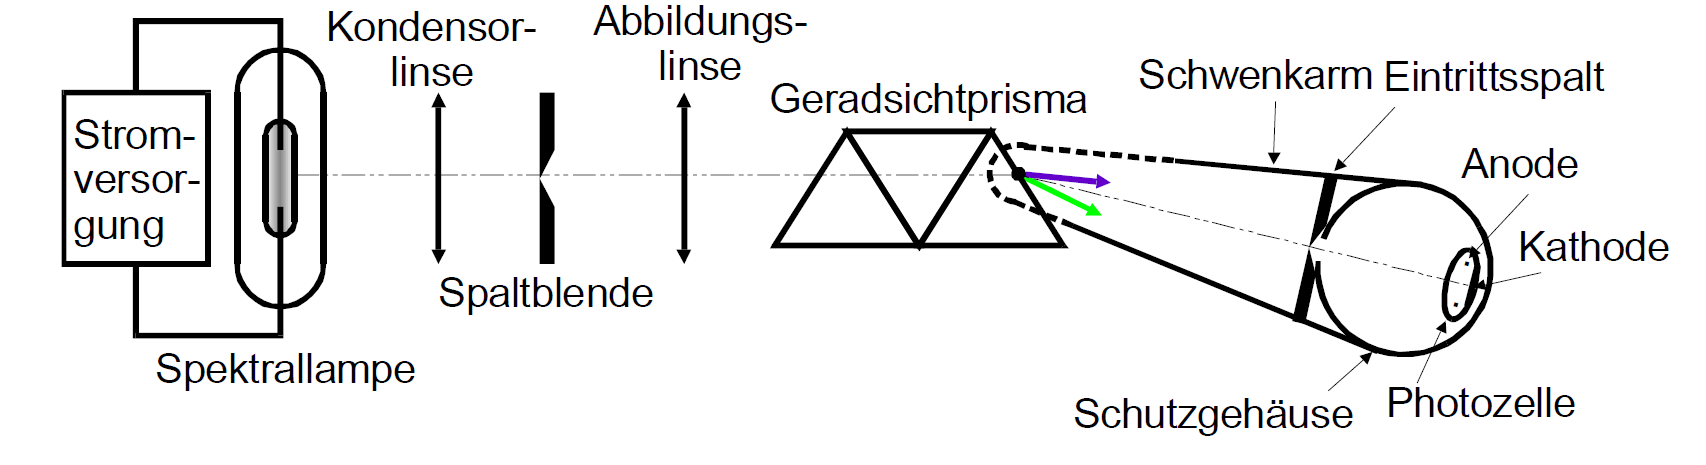
\includegraphics[width=15cm]{Bilder/Versuchsaufbau.png}
    \caption{Verwendeter Versuchsaufbau in beiden Teilversuchen (optischer Teil).\cite{sample}}
    \label{Abb:Versuchsaufbau}
\end{figure}

Die Quecksilber-Spektrallampe wird mit Strom versorgt und erzeugt Licht mit einem für Quecksilber
spezifischen Spektrum. Diese spezifischen Frequenzen sind in \autoref{Tab:HG_Spektrum} abzulesen.

\begin{figure}
    \centering
    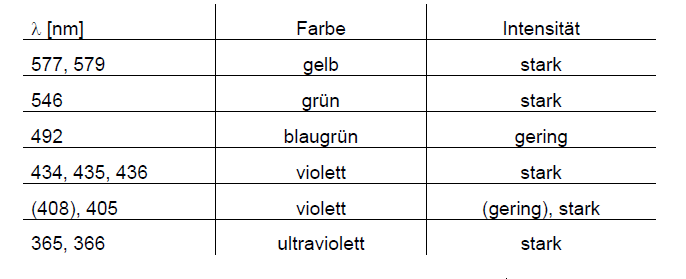
\includegraphics[width=15cm]{Bilder/Hg_Spektrum.png}
    \caption{Die dominantesten Linien im Hg-Spektrum.\cite{sample}}
    \label{Tab:HG_Spektrum}
\end{figure}

Das erzeugte Licht wird in der Kondensorlinse gebündelt und fällt auf die Spaltblende. 
Die danach geschaltete Abbildungslinse entwirft nun ein Bild der Spaltblendenöffnung
auf den Eintrittsspalt der Photokathode.\\
Danach durchläuft das Licht ein Geradsichtprisma, wodurch die einzelnen enthaltenen Frequenzen
optisch getrennt werden. Somit sind auf der Mattscheibe vor der Photokathode nun die einzelnen
Spektallinien zu beobachten.\\
Die Kathode kann nun mit einem Schwenkarm so geschwenkt werden, sodass jeweils nur eine 
Spektrallinie auf den Eintrittsspalt fällt.\\
Um Gegenfelder und Beschleunigungssfelder zu erzeugen und den Strom zu messen, wird außerdem
der in \autoref{Abb:StromZeug} verwendete Versuchsaufbau verwendet.

\begin{figure}
    \centering
    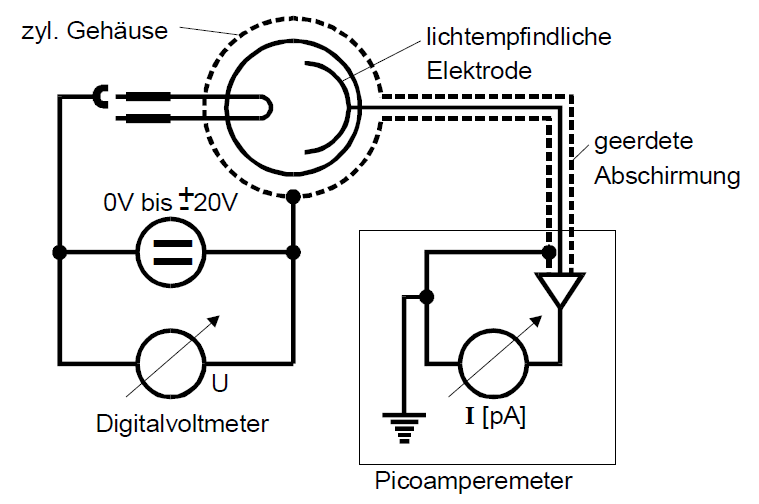
\includegraphics[width=15cm]{Bilder/StromZeug.png}
    \caption{Verwendeter Versuchsaufbau in beiden Teilversuchen (elektrisches Schaltbild).\cite{sample}}
    \label{Abb:StromZeug}
\end{figure}
